\section{Measure}

\begin{definition}[Measure]
    Suppose $(X,\mathcal{A})$ is a measurable space. A \textit{measure} on $(X,\mathcal{A})$ is a function $\mu:\mathcal{A}\to[0,\infty]$ such that
    \begin{enumerate}
        \item $\mu(\emptyset)=0$
        \item For every disjoint sequence of sets $\{E_k\}$ in  $\mathcal{A}$.
            \[
                \mu\left( \bigcup_{k=1}^{\infty}E_k \right) = \sum_{k=1}^{\infty}\mu(E_K)
            \]
    \end{enumerate}
\end{definition}

\begin{example}[]
    \  
    \begin{itemize}
        \item If $X$ is a set, then  \textit{counting measure} is a measure $\mu$ defined on the \sig-algebra of all subsets of  $X$ by 
            \[
                \mu(E)= 
                \begin{cases}
                    n \ \ \ \ &\text{if} \ E\ \text{is a finite set containing exactly n element.}\\
                    \infty\ &\text{if} \ E\ \text{is not a finite set.}
                \end{cases}
            \]
        \item $(X,\mathcal{A})$ is a measurable space and $c\in X$. Define the  \textit{Dirac measure} $\delta_c$ on  $(X,\mathcal{A})$ by
            \[
                \delta_c(E)=
                \begin{cases}
                    1 \ \text{if}\ c\in E,\\
                    0 \ \text{if}\ c\notin E.
                \end{cases}
            \]
        \item Let, $\Omega$ is sample space and $\Sigma$ is \sig-algebra on  $\Omega$. Then $P:\Sigma\to[0,1]$  is a measure on $(\Omega,\Sigma)$ such that  
            $P(\Omega)=1$ then, $P$ is called probability measure and $(\Omega,\Sigma,P)$ is called probability space.
    \end{itemize}
\end{example}

\begin{definition}[measure space]
    A measure space is an ordered triple $(X,\mathcal{A},\mu)$, where $X$ is a nonempty set,  $\mathcal{A}$ is a \sig-algebra on $X$, and  $\mu$ is a measure on  $(X,\mathcal{A})$.
\end{definition}

%%%%%%%%%%%%%%%%%%%%%%%%%%%%
\subsection*{Properties of measure}

\begin{theorem}[measure preserves order or monotonic property]
    \label{minus pro}
    Suppose $(X,\mathcal{A},\mu)$ is a measure space and $D,E\in\mathcal{A}$ are such that $D\subset E$. Then,
    \begin{enumerate}
        \item $\mu(D)\le \mu(E)$,
        \item $\mu(E\setminus D)=\mu(E)-\mu(D)$ provided that $\mu(D)<\infty$.
    \end{enumerate}
\end{theorem}
\begin{proof}
    We have $E=D\cup(E\setminus D)$ and this is a disjoint union
    \begin{equation}
        \label{muE}
        \mu(E) = \mu(D) + \mu(E\setminus D) \ge \mu(D).
    \end{equation}
    which proves (1).\\
    If $\mu(D)<\infty$, Then subtracting $\mu(D)$ from both side of equation (\refeq{muE}) proves (2) also.
\end{proof}

\begin{theorem}[]
    Suppose $(X,\mathcal{A},\mu)$ is a measure space and $\{E_k\}\in\mathcal{A}\ \forall\ k\in \mathds{N}$. Then,
    \[
        \mu \left( \bigcup_{k=1}^{\infty}E_k \right)\le \sum_{k=1}^{\infty}\mu(E_k). 
    \]
\end{theorem}
\begin{proof}
    Let, $D_1=\emptyset$ and $D_k=E_1\cup \ldots\cup E_k$ for $k\ge 2$. Then,
    \[
        E_1\setminus D_1,E_2\setminus D_2,E_3\setminus D_3,\ldots
    \]
    is a disjoint sequence of subsets of $X$ whose union equals  $\cup_{k=1}^{\infty}E_k$. Thus
    \begin{align*}
        \mu\left( \bigcup_{k=1}^{\infty}E_k \right) &= \mu\left( \bigcup_{k=1}^{\infty}(E_k\setminus D_k) \right)\\
                                                    &= \sum_{k=1}^{\infty} \mu(E_k\setminus D_k)\\
                                                    &\le \sum_{k=1}^{\infty}\mu(E_k) \ \ \text{ (By theorem \refeq{minus pro})}
    \end{align*}
    This proves the result.
\end{proof}

\begin{theorem}
    \label{increasing}
    Suppose $(X,\mathcal{A},\mu)$ is a measure space and $E_1\subset E_2\subset\ldots$ is an increasing sequence of sets in $\mathcal{A}$. Then
    \[
        \mu\left( \bigcup_{k=1}^{\infty}E_k \right) = \lim_{n\to\infty}\mu(E_k).
    \]
\end{theorem}
\begin{proof}
    \
    \begin{center}
        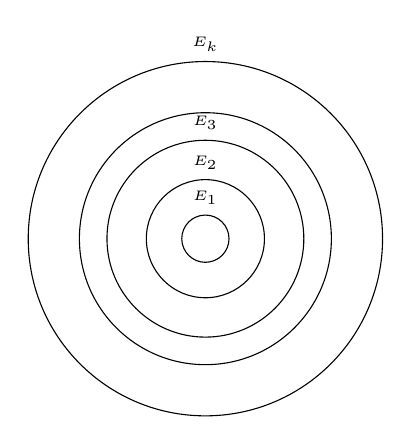
\begin{tikzpicture}
            \node[draw, circle, minimum size =6mm, label=\tiny{$E_1$}] (circle1) at (0,0){};
            \node[draw, circle, minimum size =1.5cm, label=\tiny{$E_2$}] (circle2) at (0,0){};
            \node[draw, circle, thin , minimum size =2.5cm, label=\tiny{$E_3$}] (circle3) at (0,0){};
            \node[draw, circle, thin , minimum size =3.2cm] (circle3) at (0,0){};
            \node[draw, circle, minimum size =4.5cm, label=\tiny{$E_k$}] (circle4) at (0,0){};
        \end{tikzpicture}
    \end{center}
    If $\mu(E_k)=\infty$ for some $k\in\mathds{N}$, then the equitation above is holds because both side equal $\infty$. Hence we can consider only the case where
    $\mu(E_k)<\infty\ \ \forall\ k\in\mathds{N}$.

    For convenience, let $E_0=\emptyset$. Then,
    \[
        \bigcup_{k=1}^{\infty}E_k=\bigcup_{j=1}^{\infty}(E_j\setminus E_{j-1})
    \]
    Where union on the right side is a disjoint union. Thus,

    \begin{align*}
        \mu\left( \bigcup_{k=1}^{\infty}E_k \right) &= \sum_{j=1}^{\infty}\mu(E_j\setminus E_{j-1})\\
                                                    &= \lim_{k\to\infty}\sum_{j=1}^{k}\mu(E_j\setminus E_{j-1})\\
                                                    &= \lim_{k\to\infty}\sum_{j=1}^{k}\left( \mu(E_j)-\mu(E_{j-1}) \right)\\
                                                    &= \lim_{k\to\infty}\mu(E_k).
    \end{align*}
    Hence proved.
\end{proof}

\begin{theorem}[]
    Suppose $(X,\mathcal{A},\mu)$ is a measure space and $E_1\supset E_2\supset\ldots$ is a decreasing sequence of sets in $\mathcal{A}$, with $\mu(E_1)<\infty$. Then
    \[
        \mu\left( \bigcap_{k=1}^{\infty}E_k \right) = \lim_{k\to\infty}\mu(E_k).
    \]
\end{theorem}
\begin{proof}
    By De Morgan's law we have,
    \[
        E_1\setminus \bigcap_{k=1}^{\infty}E_k = \bigcup_{k=1}^{\infty}(E_1\setminus E_k).
    \]
    Now $E_1\setminus E_1,\ E_1\setminus E_2,\ E_1\setminus E_3$ is an increasing sequence of sets in $\mathcal{A}$.
    Thus, by \refeq{increasing},
    \begin{align*}
        \mu\left(E_1\setminus \bigcap_{k=1}^{\infty}E_k\right) &= \lim_{k\to\infty}\mu(E_1\setminus E_k)\\
        \mu\left(E_1\setminus \bigcap_{k=1}^{\infty}E_k\right) &= \lim_{k\to\infty}\left( \mu(E_1)-\mu(E_k) \right) \\
        \mu(E_1)-\mu\left( \bigcap_{k=1}^{\infty}E_k \right) &= \mu(E_1)-\lim_{k\to\infty}\mu(E_k)\\
        \mu\left( \bigcap_{k=1}^{\infty}E_k \right) &= \lim_{k\to\infty}\mu(E_k)
    \end{align*}
\end{proof}
\begin{theorem}[measure of union]
    Suppose $(X,\mathcal{A},\mu)$ is a measure space and $D,E\in\mathcal{A}$, with $\mu(D\cap E)<\infty$. Then
    \[
         \mu(D\cup E)=\mu(D)+\mu(E)-\mu(D\cap E).
    \]
\end{theorem}
\begin{proof}
    We have 
    \[
        D\cup E=(D\setminus (D\cap E))\cup(E\setminus (D\cap E))\cup(D\cap E)
    \]
    where every sets in right side are disjoint so from properties of measure,
    \begin{align*}
        \mu(D\cup E)&=\mu(D\setminus (D\cap E)) + \mu(E\setminus (D\cap E)) + \mu(D\cap E)\\
                    &=\mu(D) - \mu(D\cap E) + \mu(E) - \mu(D\cap E) + \mu(D\cap E)\\
                    &=\mu(D)+\mu(E)-\mu(D\cap E).
    \end{align*}
    Hence proved.
\end{proof}
